\documentclass[11pt,a4paper]{article}
\usepackage[margin=2.5cm]{geometry}
\usepackage[T1]{fontenc}
\usepackage{lmodern}
\usepackage{microtype}
\usepackage{amsmath,amssymb}
\usepackage{graphicx}
\usepackage{booktabs}
\usepackage{float}
\usepackage{caption}
\usepackage{enumitem}
\usepackage{xcolor}
\usepackage[colorlinks=true,linkcolor=blue!50!black,citecolor=blue!50!black,urlcolor=blue!50!black]{hyperref}
\graphicspath{{../../figures/}}
\newcommand{\tabCa}{%
Model & $H=1$ & $H=25$ & $H=100$ & Energy drift, $t=200$ \\ \midrule
Physics & $2.5\times 10^{-6}$ & $2.5\times 10^{-5}$ & $1.1\times 10^{-4}$ & $5.2\times 10^{-6}$ \\
Neural Hamiltonian & $2.9\times 10^{-5}$ & $1.7\times 10^{-4}$ & $6.7\times 10^{-4}$ & $7.5\times 10^{-5}$ \\
MLP ensemble & $4.3\times 10^{-5}$ & $7.2\times 10^{-4}$ & $4.9\times 10^{-3}$ & $4.1\times 10^{-3}$ \\
Physics + residual & $1.3\times 10^{-4}$ & $1.5\times 10^{-3}$ & $7.0\times 10^{-3}$ & $3.0\times 10^{-3}$ \\
Neural ODE & $1.3\times 10^{-4}$ & $2.4\times 10^{-3}$ & $2.0\times 10^{-2}$ & $3.3\times 10^{-2}$ \\
Legacy latent ODE & $5.2\times 10^{-4}$ & $8.4\times 10^{-3}$ & $5.9\times 10^{-2}$ & $5.9\times 10^{-2}$ \\%
}
\newcommand{\tabCb}{%
Model & 400 transitions & 1000 transitions & 5000 transitions \\ \midrule
Physics & $1.0\times 10^{-4}$ & $5.8\times 10^{-4}$ & $1.1\times 10^{-4}$ \\
Neural Hamiltonian & $9.1\times 10^{-4}$ & $8.2\times 10^{-4}$ & $6.7\times 10^{-4}$ \\
MLP ensemble & $1.0\times 10^{-2}$ & $9.5\times 10^{-3}$ & $4.9\times 10^{-3}$ \\
Physics + residual & $8.6\times 10^{-3}$ & $9.3\times 10^{-3}$ & $7.0\times 10^{-3}$ \\
Neural ODE & $4.3\times 10^{-2}$ & $2.0\times 10^{-2}$ & $2.0\times 10^{-2}$ \\
Legacy latent ODE & $1.4\times 10^{-1}$ & $7.2\times 10^{-2}$ & $5.9\times 10^{-2}$ \\%
}
\newcommand{\tabD}{%
Method & Return, last three episodes (mean and 95\% CI) & Seeds solved \\ \midrule
Physics & $-382$ $[-390,\ -375]$ & 5 of 5 \\
Physics + residual & $-382$ $[-390,\ -375]$ & 5 of 5 \\
Neural Hamiltonian & $-382$ $[-389,\ -375]$ & 5 of 5 \\
MLP ensemble & $-382$ $[-390,\ -376]$ & 5 of 5 \\
Neural ODE & $-382$ $[-388,\ -375]$ & 5 of 5 \\
Legacy latent ODE & $-381$ $[-388,\ -375]$ & 5 of 5 \\
SAC & $-522$ $[-673,\ -373]$ & 3 of 5 \\%
}
\newcommand{\tabL}{%
Model & 50 transitions & 100 transitions & 200 transitions \\ \midrule
Physics & 5 of 5 ($\bar R=-382$) & 5 of 5 ($\bar R=-382$) & 5 of 5 ($\bar R=-381$) \\
Physics + residual & 5 of 5 ($\bar R=-384$) & 5 of 5 ($\bar R=-360$) & 5 of 5 ($\bar R=-382$) \\
Neural Hamiltonian & 5 of 5 ($\bar R=-361$) & 5 of 5 ($\bar R=-381$) & 5 of 5 ($\bar R=-381$) \\
MLP ensemble & 3 of 5 ($\bar R=-675$) & 2 of 5 ($\bar R=-759$) & 5 of 5 ($\bar R=-381$) \\
Neural ODE & 4 of 5 ($\bar R=-449$) & 2 of 5 ($\bar R=-703$) & 5 of 5 ($\bar R=-360$) \\
Legacy latent ODE & 1 of 5 ($\bar R=-995$) & 0 of 5 ($\bar R=-1405$) & 4 of 5 ($\bar R=-406$) \\%
}
\newcommand{\tabEa}{%
Shift & Oracle & Unadapted (physics) & Physics & Physics + residual & Neural Hamiltonian & MLP ensemble & Neural ODE & Legacy latent ODE \\ \midrule
$g \times 0.5$ & $-227$ & $-517$ & $-206$ & $-206$ & $-206$ & $-236$ & $-229$ & $-244$ \\
$g \times 1.5$ & $-449$ & $-1260$ & $-443$ & $-443$ & $-453$ & $-456$ & $-490$ & $-477$ \\
$g \times 2.0$ & $-556$ & $-1507$ & $-568$ & $-567$ & $-607$ & $-682$ & $-681$ & $-1036$ \\
$l \times 0.7$ & $-252$ & $-257$ & $-245$ & $-245$ & $-246$ & $-249$ & $-248$ & $-245$ \\
$l \times 1.5$ & $-578$ & $-1049$ & $-585$ & $-585$ & $-587$ & $-584$ & $-580$ & $-591$ \\
$m \times 0.5$ & $-208$ & $-237$ & $-210$ & $-211$ & $-213$ & $-217$ & $-217$ & $-221$ \\
$m \times 2.0$ & $-630$ & $-861$ & $-639$ & $-639$ & $-652$ & $-663$ & $-652$ & $-692$ \\%
}
\newcommand{\tabEb}{%
Model & 25 & 50 & 100 & 200 & 500 & 1000 \\ \midrule
Physics & $1.9\times 10^{-10}$ & $1.7\times 10^{-10}$ & $1.2\times 10^{-10}$ & $1.7\times 10^{-10}$ & $1.6\times 10^{-10}$ & $1.7\times 10^{-10}$ \\
Neural Hamiltonian & $5.5\times 10^{-2}$ & $3.7\times 10^{-3}$ & $5.1\times 10^{-4}$ & $3.5\times 10^{-4}$ & $3.4\times 10^{-4}$ & $3.2\times 10^{-4}$ \\
MLP ensemble & $1.6\times 10^{-1}$ & $3.9\times 10^{-2}$ & $3.8\times 10^{-3}$ & $2.9\times 10^{-3}$ & $1.8\times 10^{-3}$ & $1.8\times 10^{-3}$ \\
Neural ODE & $1.7\times 10^{-1}$ & $5.2\times 10^{-2}$ & $7.9\times 10^{-3}$ & $4.8\times 10^{-3}$ & $2.9\times 10^{-3}$ & $2.8\times 10^{-3}$ \\
Legacy latent ODE & $3.0\times 10^{-1}$ & $6.4\times 10^{-2}$ & $2.7\times 10^{-2}$ & $1.8\times 10^{-2}$ & $1.3\times 10^{-2}$ & $1.3\times 10^{-2}$ \\%
}
\newcommand{\recovAmed}{$1.9\times 10^{-10}$}
\newcommand{\recovAmax}{$5.5\times 10^{-10}$}
\newcommand{\recovCmed}{$4.6\times 10^{-10}$}
\newcommand{\recovCmax}{$2.2\times 10^{-9}$}
\newcommand{\recovN}{35}
\newcommand{\tabF}{%
Model & Return, last three episodes & Prediction error at $H=25$ \\ \midrule
Oracle (true simulator) & $-640$ $[-651,\ -629]$ & not applicable \\
Physics, no friction term & $-673$ $[-724,\ -625]$ & $2.8\times 10^{-1}$ $[2.8\times 10^{-1},\ 2.8\times 10^{-1}]$ \\
Physics, no friction term + residual & $-639$ $[-650,\ -629]$ & $6.2\times 10^{-3}$ $[4.1\times 10^{-3},\ 8.5\times 10^{-3}]$ \\
Physics & $-631$ $[-643,\ -623]$ & $8.1\times 10^{-2}$ $[3.2\times 10^{-2},\ 1.3\times 10^{-1}]$ \\
Neural Hamiltonian & $-638$ $[-656,\ -619]$ & $2.7\times 10^{-1}$ $[2.6\times 10^{-1},\ 2.8\times 10^{-1}]$ \\
MLP ensemble & $-638$ $[-646,\ -630]$ & $7.1\times 10^{-3}$ $[6.3\times 10^{-3},\ 7.9\times 10^{-3}]$ \\
Neural ODE & $-644$ $[-654,\ -633]$ & $8.6\times 10^{-3}$ $[7.1\times 10^{-3},\ 1.0\times 10^{-2}]$ \\%
}

\hyphenpenalty=10000\exhyphenpenalty=10000\sloppy
\setlength{\parskip}{0.5em}
\setlength{\parindent}{0pt}
\captionsetup{font=small,labelfont=bf}
\newcommand{\R}{\mathbb{R}}

\title{Physics Informed World Models for Control\\[0.3em]\large An Extension of the Orbit Study to Model Based Control of a Pendulum}
\author{Aditya Raj}
\date{November 2026}

\begin{document}
\maketitle

\begin{abstract}
My earlier project showed that a physics informed latent neural ODE can stay on a bounded orbit far beyond its training window (though its timing drifts), but that model had no control input, so it said nothing about control. This report is the extension. I ask whether building physics structure into a learned world model helps a model based agent learn to control a system with less data, and whether the agent keeps working when gravity, length or mass change at test time. I compare six world models (an MLP ensemble, a plain neural ODE, a structured physics model with and without a neural residual, a neural Hamiltonian with control in the style of Symplectic ODE Net, and my earlier latent ODE adapted to take actions) on a pendulum swing up task, using a batched MPPI planner and SAC as a model free reference. Everything is simulation, noise free, state based, with five seeds per setting. The results are mixed and I report them as they are. Structure clearly helps prediction: the physics model reaches a one hundred step error of about $10^{-4}$ and, after fifty new transitions, an error near $10^{-10}$ in a shifted world, which no black box matched even with one thousand transitions. Structure helps much less for control return. All models solve the task from five hundred random transitions, and after adaptation all models land close to an oracle planner. Only at fifty to one hundred transitions did the structured models solve the task more reliably. With unmodelled friction and a hidden motor limit the physics model fails to predict, and a learned residual repairs it only to the level of a plain MLP. The code, raw results and tests are in the repository.
\end{abstract}

\tableofcontents
\newpage

%--------------------------------------------------------------------
\section{Introduction}
The first part of this repository studied a two body orbit. A plain neural network spiralled away from the true orbit, a physics informed neural network lost phase over long horizons, and a latent neural ODE with an energy variance penalty stayed on a bounded orbit over a window twenty five times longer than its training data, although its orbital period was slightly off, so its position drifted (see \texttt{docs/ERRATA\_PART\_I.md}). That was a prediction problem. A world model is only useful for an agent if it supports decisions, and nothing in that orbit model could accept an action. I also have to be honest about one more point: its physics entered only through a soft penalty on energy variance, so it was never a Hamiltonian model, and its orbit results do not carry over to control.

This report asks the control version of the question.

\begin{quote}
Does building physics structure into a learned world model let a model based agent (a) learn to control a system with less data, and (b) keep working when the physical parameters change at test time, by estimating a handful of interpretable parameters again from a few new transitions?
\end{quote}

I tested four hypotheses, and I took seriously that any of them might be false.
\begin{description}[leftmargin=2.2em,style=nextline]
\item[H1] Physics informed models are more sample efficient than a plain MLP ensemble.
\item[H2] After a change in gravity, length or mass, a physics informed model adapts from about fifty new transitions by re estimating parameters, while a black box cannot adapt that cheaply.
\item[H3] Physics informed long horizon rollouts are more accurate and conserve energy better when there is no friction.
\item[H4] When the real system has effects the model does not contain (friction, a motor limit), the pure physics model degrades and a learned residual repairs it.
\end{description}

\paragraph{What this report is and is not.} All learning experiments use a single system, the pendulum. I wrote simulators for a cart pole and an acrobot and tested them, and I checked that the planner swings up the cart pole with the true model, but I did not train or plan with any learned model on them. The simulator is noise free and the structured model contains exactly the right equations, which is the best case for the physics approach. Each setting uses five seeds. The method ideas are not new: I re implemented known ideas as a careful, small, reproducible comparison. Section~\ref{sec:related} says exactly what is and is not new.

%--------------------------------------------------------------------
\section{Background}

\subsection{The pendulum from the Lagrangian and the Hamiltonian}
The pendulum is a uniform rod of mass $m$ and length $l$ pivoted at one end, and $\theta$ is measured from the upright position, so $\theta=0$ is the unstable equilibrium. The moment of inertia about the pivot is $I=ml^2/3$. The kinetic energy is $T=\tfrac12 I\dot\theta^2$ and the potential energy is $V=\tfrac12 mgl\cos\theta$, because the centre of mass sits at height $l/2\cdot\cos\theta$ above the pivot. The Lagrangian is $L=T-V$. With a torque $u$ and viscous friction $b\dot\theta$ acting as generalised force, the Euler Lagrange equation $\frac{d}{dt}\frac{\partial L}{\partial\dot\theta}-\frac{\partial L}{\partial\theta}=u-b\dot\theta$ gives
\begin{equation}
I\ddot\theta=\tfrac12 mgl\sin\theta+u-b\dot\theta
\quad\Longleftrightarrow\quad
\ddot\theta=\frac{3g}{2l}\sin\theta+\frac{3(u-b\dot\theta)}{ml^2}.
\label{eq:pend}
\end{equation}
This is exactly the equation used by Gymnasium's Pendulum environment~\cite{towers2024gymnasium}, and I checked the two numerically in the test suite.

The Hamiltonian form uses the momentum $p=\partial L/\partial\dot\theta=I\dot\theta$ and the total energy $H(\theta,p)=p^2/(2I)+\tfrac12 mgl\cos\theta$. Hamilton's equations are $\dot\theta=\partial H/\partial p$ and $\dot p=-\partial H/\partial\theta+u$. Two properties follow directly. With $u=0$ and no friction, $dH/dt=\frac{\partial H}{\partial\theta}\dot\theta+\frac{\partial H}{\partial p}\dot p=0$, so energy is conserved for any function $H$. And the flow preserves phase space volume, because $\frac{\partial\dot\theta}{\partial\theta}+\frac{\partial\dot p}{\partial p}=\frac{\partial^2H}{\partial\theta\partial p}-\frac{\partial^2H}{\partial p\partial\theta}=0$. A model that learns an arbitrary scalar $H(q,p)$ and integrates Hamilton's equations inherits both properties by construction. That is the idea of Symplectic ODE Net~\cite{zhong2020symoden}, closely related to Hamiltonian neural networks~\cite{greydanus2019hnn}. Standard references for the mechanics are Goldstein et al.~\cite{goldstein2002}.

\subsection{Identifiability}
Equation~\eqref{eq:pend} depends on the parameters only through $a=3g/(2l)$, $c=3/(ml^2)$ and $d=3b/(ml^2)$. There are three physical unknowns $(m,l,g)$ but only two constraints on them from state and action data, so $m$, $l$ and $g$ cannot be recovered separately. I saw this directly. Starting from wrong initial values, the structured model fits the data perfectly with $(m,l,g)=(1.66,\,0.78,\,7.76)$ while the truth is $(1,\,1,\,10)$, and yet $a=15.0$ and $c=3.0$ match the truth. So throughout this report, parameter recovery means recovering $a$ and $c$. When mass and length are held at their true values, gravity alone is recovered to within two percent (this is a unit test).

\subsection{Neural ODEs, RK4, and why rollouts drift}
A neural ODE models $\dot x=f_\theta(x,u)$ with a network $f_\theta$ and predicts the next state by numerically integrating over one control interval~\cite{chen2018neuralode}. I use the classical fourth order Runge Kutta method with the action held constant over the interval. Long rollouts drift because every step starts from the previous step's error, and for unstable dynamics such as an inverted pendulum those errors grow exponentially. Even the true equations drift if integrated too coarsely: with one RK4 step per $0.05$ seconds the energy of the true pendulum drifted by $1.4\times10^{-3}$ over one thousand steps, and four substeps brought it to $10^{-6}$. Halving the step reduced the drift by a factor of about thirty two each time, which is how I knew it was truncation error and not a mistake in the equations. Energy conserving structure removes drift in the energy direction, but not phase error.

\subsection{Model predictive control and MPPI}
Model predictive control uses a model to find a good sequence of actions over a horizon, executes only the first action, observes the real state, and plans again. Replanning from the observed state supplies feedback, which will matter for interpreting the results.

MPPI~\cite{williams2017mppi,williams2016aggressive} samples $N$ perturbed action sequences $A_i=U+\varepsilon_i$ with $\varepsilon_i\sim\mathcal N(0,\sigma^2 I)$ and rolls each through the model to obtain a return $R_i$. In the information theoretic view, the optimal control distribution under a KL regularised objective with temperature $\lambda$ reweights samples by $\exp(R_i/\lambda)$. The update is
\begin{equation}
w_i=\frac{\exp\!\big((R_i-\max_j R_j)/\lambda\big)}{\sum_k\exp\!\big((R_k-\max_j R_j)/\lambda\big)},\qquad
U\leftarrow U+\sum_{i=1}^N w_i\,\varepsilon_i .
\end{equation}
In words, the plan moves towards the noise directions that happened to score well, more strongly for much better samples. A small $\lambda$ nearly copies the best sample and a large $\lambda$ nearly averages everything. Subtracting the maximum return is only for numerical stability. Two details in my implementation matter: the unperturbed nominal plan is always one of the candidates, and the update uses the perturbation that was actually evaluated after clipping the actions to the allowed range.

\subsection{System identification from a few transitions}
Estimating parameters again from fifty transitions means solving the small nonlinear least squares problem
\begin{equation}
\min_{\vartheta}\ \sum_{i=1}^{50}\big\|x_{i+1}-\mathrm{RK4}(x_i,u_i;\vartheta)\big\|^2 ,
\end{equation}
where $\vartheta$ holds one to three physical parameters, stored as logarithms so they stay positive, and everything else is frozen. I solve it with Adam~\cite{kingma2015adam}. When the structure is exactly right and the data are noise free, fifty transitions are plenty. Black box models are instead fine tuned on all their weights using the same transitions.

\subsection{Statistics with few seeds}
With five seeds a normal interval is unreliable, so I report percentile bootstrap intervals~\cite{efron1979bootstrap}, which resample the seeds with replacement five thousand times, and the interquartile mean, which averages the middle half of the values, as recommended by Agarwal et al.~\cite{agarwal2021precipice}. With five points even the bootstrap interval is rough and somewhat too narrow, so I treat intervals as a description of spread and not as proof.

%--------------------------------------------------------------------
\section{What I built}

\subsection{What existed before and what is new}
\begin{table}[H]
\centering\small
\begin{tabular}{p{6.2cm}p{8.2cm}}
\toprule
Existing in the repository & New in the control extension \\
\midrule
\texttt{src/dynamics.py}: NumPy RK4 and the orbit equations & \texttt{src/control/envs/}: batched torch RK4, pendulum, cart pole, acrobot, Gymnasium bridge \\
\texttt{src/models.py}: encoder, dopri5 neural ODE, decoder, energy variance loss (no actions, not Hamiltonian) & \texttt{src/control/models/}: MLP ensemble, neural ODE, structured physics, residual, neural Hamiltonian, legacy latent ODE with actions \\
\texttt{src/train\_*.py}, \texttt{data/generate\_orbit.py} & \texttt{src/control/eval/}: data collection, trainer, rollout and energy metrics, bootstrap statistics \\
\texttt{tests/test\_dynamics.py} & \texttt{tests/}: simulator, planner, model, statistics and adaptation tests (38 in total) \\
\texttt{requirements.txt}, README, \texttt{report.pdf}, \texttt{assets/} & planners, agents (MBRL loop and SAC), \texttt{adapt/sysid.py}, \texttt{experiments/}, \texttt{analysis/}, \texttt{demo/}, \texttt{docs/} \\
\bottomrule
\end{tabular}
\caption{Division between the earlier orbit work and the control extension. The orbit code, its report and its figures are untouched, and its unit test still passes.}
\end{table}

\subsection{Simulators}
The pendulum uses equation~\eqref{eq:pend}. The cart pole uses a point mass on a massless rod, with the two Euler Lagrange equations solved for the cart acceleration and the pole acceleration. The acrobot is a double pendulum with torque only at the second joint, written in manipulator form. Each simulator is batched in PyTorch in double precision, integrates with RK4 and a zero order hold on the action, and lets me change parameters at test time. I chose the number of RK4 substeps (four for the pendulum and cart pole, eight for the acrobot) from the energy convergence test described above. Gymnasium's Pendulum environment was used as an independent cross check, not as the engine, because it uses Euler steps, single precision and fixed length episodes. The cross check matched the acceleration to float32 precision.

\subsection{World models}
All models predict the next state from a state and an action and use one common training recipe, so differences come from the model class and not from the optimiser. Angles enter every network as cosine and sine pairs.
\begin{itemize}[leftmargin=1.5em]
\item \textbf{MLP ensemble.} Five members with three hidden layers of 200 units, trained on state increments with bootstrap weights and a mean squared error loss (not the Gaussian likelihood of PETS~\cite{chua2018pets}). Planning uses the member mean.
\item \textbf{Neural ODE.} A network gives the state derivative and RK4 integrates it, with no physics inside.
\item \textbf{Structured physics.} The analytic equations of the simulator with learnable $m$, $l$, $g$ and $b$ (stored as logarithms for positivity). I start these from the truth multiplied by a random factor between $0.6$ and $1.4$, and the friction starts at zero. An optional residual network is added to the derivative, with its output layer initialised near zero and an L2 penalty, in the spirit of APHYNITY~\cite{yin2021aphynity} (I do not use their constrained optimisation).
\item \textbf{Neural Hamiltonian with control.} A re implementation in my own style of the structure of Symplectic ODE Net~\cite{zhong2020symoden}: a potential $V(q)$, an inverse mass matrix $M^{-1}(q)=LL^\top+\epsilon I$ and an input matrix $g(q)$, all small networks. Data come as positions and velocities, so the model converts to momenta with its own learned mass matrix, integrates Hamilton's equations with RK4 using automatic differentiation of $H$, and converts back. It has no dissipation term, so friction is outside what it can represent, on purpose.
\item \textbf{Legacy latent ODE.} The model from Part I (encoder, dopri5 ODE through torchdiffeq~\cite{chen2018neuralode}, decoder; tanh layers, 64 hidden units). To use it for control I had to change three things: the ODE now receives the action, the decoder predicts a residual from the current state because an absolute state decoder cannot resolve one step increments, and I dropped the orbit specific energy penalty. I want to be clear that this model was never Hamiltonian and was designed to fit one trajectory.
\end{itemize}
Training is Adam with learning rate $10^{-3}$, batch size 256, at most 1500 steps, early stopping on a validation split taken by episode, and the best validation weights restored. The loss is the one step squared error divided by the standard deviation of the state increment.

\subsection{The control loop, adaptation and SAC}
The model based agent first collects ten random episodes of fifty transitions, fits the model, then repeats the following ten times: plan two hundred steps with MPPI in the model while the true simulator executes the actions, add the new transitions to the data, and refit starting from the current weights. The reward function is known to the agent and only the dynamics are learned. Planner settings found with the true simulator (forty steps horizon, four hundred to five hundred samples, $\lambda=0.5$, $\sigma=1$) are used throughout.

For adaptation, fifty new transitions (five episodes of ten steps with random actions) are collected in the shifted world. The structured model freezes everything except its physical parameters. The black boxes are fine tuned on all weights with early stopping on a held out episode, and their learning rate was chosen from a small grid on a separate tuning shift (gravity times $0.75$ and length times $1.2$), so they are tuned fairly.

SAC~\cite{haarnoja2018sac} is structured after the single file implementation in CleanRL~\cite{huang2022cleanrl} (tanh Gaussian actor, twin critics, automatic entropy tuning), run on the same simulator with deterministic evaluation episodes every five hundred steps.

\subsection{Verification before any learning}
Three gates had to pass before I trusted anything learned.
\begin{itemize}[leftmargin=1.5em]
\item \textbf{Gate A, simulators.} Energy drift below $10^{-4}$ (relative) over one thousand steps with no control and no friction; PyTorch and NumPy trajectories agree to $10^{-9}$; the small oscillation period of the hanging rod matches $2\pi\sqrt{2l/(3g)}$. The prompt for this project quoted the point mass formula $2\pi\sqrt{l/g}$, but my pendulum is a rod with $I=ml^2/3$, so I tested the law that actually applies.
\item \textbf{Gate B, planner with the true model.} MPPI swings up and balances the pendulum from rest at the bottom in five of five seeds (returns between $-320$ and $-372$ over two hundred steps), a cross entropy method planner does the same, and MPPI swings up the cart pole in five of five seeds. My MPPI matches the \texttt{pytorch\_mppi} package~\cite{pytorchmppi} on the true pendulum: mean return $-358$ against $-373$, within the seed spread.
\item \textbf{Gate C, models.} All models train, produce the right shapes and gradients, and the structured model reproduces the simulator to $10^{-16}$ when given the true parameters.
\end{itemize}

%--------------------------------------------------------------------
\section{Experimental design}
Training data are random uniform actions from wide random initial states (angular speed up to eight radians per second), in episodes of fifty transitions, with the train and validation split made by episode so correlated rows cannot leak across it. Evaluation uses two hundred fixed held out trajectories generated with seeds that were never used for training. For control, episodes start near the bottom with small noise. Seeds zero to four are used everywhere, and within one seed all models see the same start states and planner seeds, so that models are compared on the same episodes. This also explains why returns of different models are often almost identical.

\begin{itemize}[leftmargin=1.5em]
\item \textbf{H1} was tested in two ways: learning curves over ten model based iterations after five hundred random transitions, and, because that turned out not to separate the models, a second sweep that fits each model on only fifty, one hundred or two hundred random transitions and measures one planning episode. I added the second sweep after seeing the first result, and I flag it as a follow up and not a plan made in advance.
\item \textbf{H2}: models trained at the default parameters were evaluated at gravity times $0.5$, $1.5$, $2$, length times $0.7$, $1.5$ and mass times $0.5$, $2$, with and without adaptation, against an oracle (MPPI that uses the true shifted simulator). I also measured prediction error as a function of the number of adaptation transitions, from twenty five to one thousand.
\item \textbf{H3}: prediction error against rollout horizon on the held out set, and drift of the true energy along model rollouts with zero control and no friction.
\item \textbf{H4}: a pendulum with viscous friction $b=0.15$ and a hidden actuator saturation at $1.5$ while the planner is allowed commands up to $2$. Every model learns from scratch inside this world. The physics model is tested with its friction frozen at zero (so the effect is unmodelled), with and without the residual, and also with a learnable friction coefficient.
\end{itemize}

\paragraph{Things I did not control.} The legacy model has a smaller network than the others. The MLP ensemble uses a squared error loss and not a likelihood. None of the models uses a multi step training loss, which probably handicaps the black boxes at long horizons. Running time differs enormously: one neural Hamiltonian run took 8762 seconds against 109 for the physics model on a busy CPU. SAC and the model based agents are matched in environment steps but not in compute. And there are only five seeds.

%--------------------------------------------------------------------
\section{Results}
All numbers below come from files in \texttt{results/}, and the figure scripts and table scripts read those files directly. The full table of means and intervals is in \texttt{results/summary\_table.md}.

\subsection{Prediction accuracy and energy conservation (H3)}
Figure~\ref{fig:horizon} shows the error against rollout horizon on the left and the drift of the true energy along model rollouts on the right, for models trained on five thousand transitions. Table~\ref{tab:C} gives the numbers.

\begin{figure}[H]
\centering
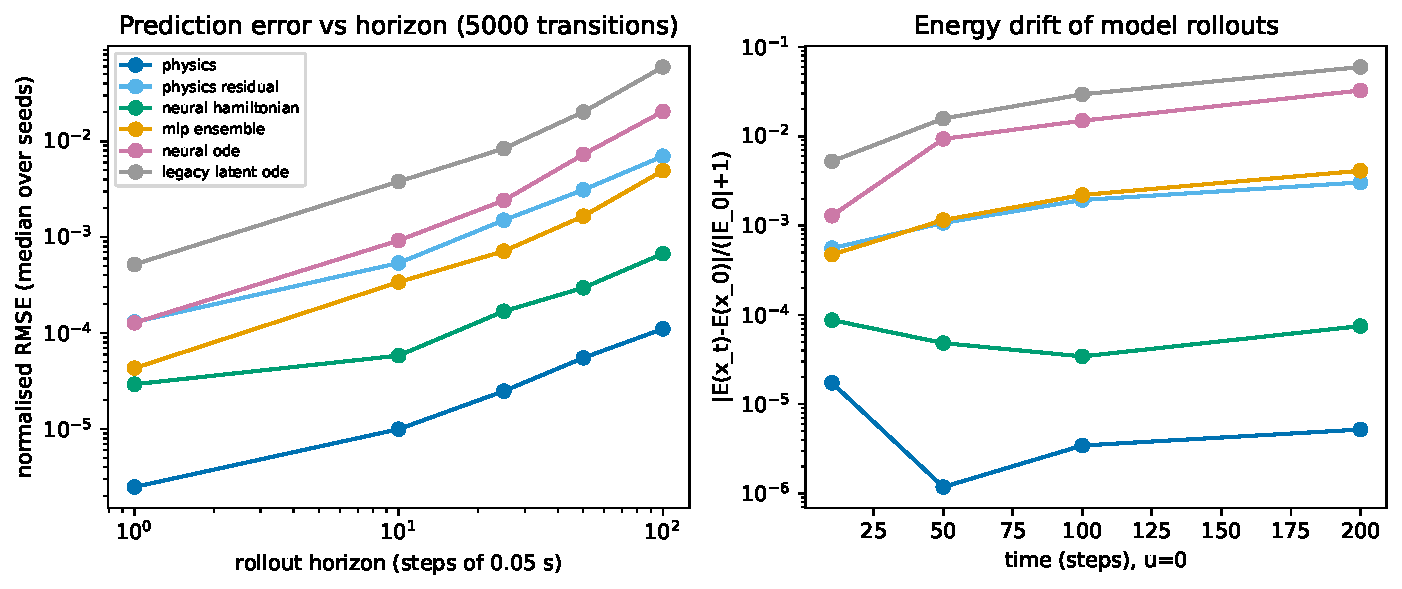
\includegraphics[width=\textwidth]{fig3_horizon_energy.pdf}
\caption{Left: median normalised RMSE against rollout horizon (steps of $0.05$ s), five seeds, lower is better. Right: relative drift of the true energy along model rollouts with zero control, where a flat curve means energy is conserved.}
\label{fig:horizon}
\end{figure}

\begin{table}[H]
\centering\small
\begin{tabular}{lcccc}
\toprule
\tabCa
\bottomrule
\end{tabular}
\caption{Median prediction error at three horizons and energy drift at step 200, models trained on 5000 transitions (source: \texttt{results/phase\_c\_pendulum.json}).}
\label{tab:C}
\end{table}

The order is the same at every horizon: physics, then neural Hamiltonian, then MLP ensemble, then neural ODE, then the legacy model. The neural Hamiltonian is the most interesting entry. It knows nothing about the pendulum's equations, yet it is within a factor of six of the exact physics model at one hundred steps and its energy drift stays flat from step ten to step two hundred, while the MLP and the neural ODE drift by two to three orders of magnitude more. The residual hurts on clean data, because it adds capacity that nothing needs. Table~\ref{tab:C2} shows that the ranking holds from 400 to 5000 transitions. The physics number at 1000 transitions is higher than at 400, which is seed to seed variance, and I did not investigate the cause further. H3 is supported.

\begin{table}[H]
\centering\small
\begin{tabular}{lccc}
\toprule
\tabCb
\bottomrule
\end{tabular}
\caption{Median prediction error at horizon 100 for three training set sizes (source: \texttt{results/phase\_c\_pendulum.json}).}
\label{tab:C2}
\end{table}

\subsection{Learning curves and sample efficiency (H1)}
\begin{figure}[H]
\centering
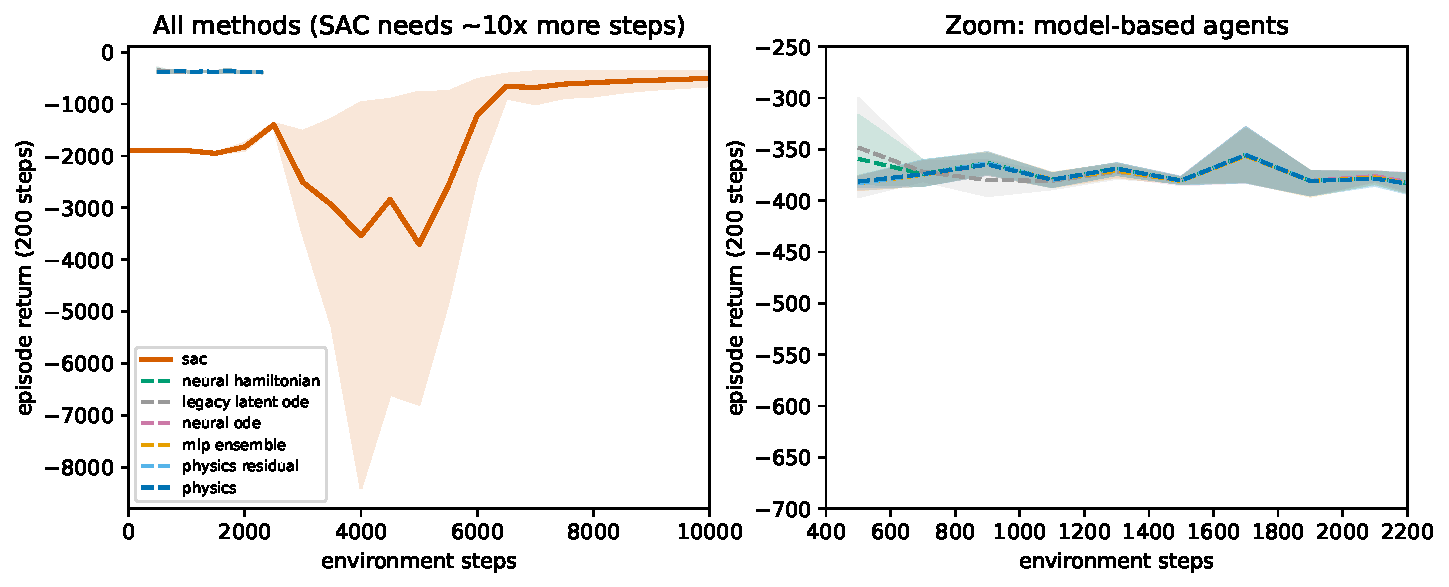
\includegraphics[width=\textwidth]{fig1_learning_curves.pdf}
\caption{Episode return (zero is best) against environment steps, mean over five seeds with 95\% bootstrap bands. Left: all methods. Right: zoom on the model based agents. A successful swing up scores about $-320$ to $-380$; an untrained policy scores about $-1900$.}
\label{fig:curves}
\end{figure}

Figure~\ref{fig:curves} is a humbling result. Every model based agent, including the weak legacy model, swings the pendulum up from its very first planning episode, after only five hundred random transitions. Their final returns agree to within a few units (Table~\ref{tab:D}). SAC needs roughly eight to ten thousand steps, and only three of five seeds had solved the task by ten thousand. So model based control was about an order of magnitude more sample efficient than SAC here, but physics structure was not the reason, since all model classes tie. At this data size H1 is neither supported nor refuted.

\begin{table}[H]
\centering\small
\begin{tabular}{lcc}
\toprule
\tabD
\bottomrule
\end{tabular}
\caption{Final return, mean of the last three episodes per seed, with the mean over five seeds and a 95\% bootstrap interval (source: \texttt{results/phase\_d\_pendulum.json}). A seed counts as solved if its return is above $-500$.}
\label{tab:D}
\end{table}

Because the main sweep could not tell the models apart, I ran the low data sweep (Figure~\ref{fig:low}, Table~\ref{tab:L}). With only fifty random transitions the physics model, the physics model with a residual and the neural Hamiltonian solved all five seeds, the MLP ensemble solved three, the neural ODE four and the legacy model one. At one hundred transitions the black boxes did worse than at fifty, which I read as noise: with only one or two random episodes the coverage of the state space is a lottery, and five seeds cannot average that out. At two hundred transitions most black boxes catch up. I regard this as suggestive evidence for H1 in the fifty to one hundred transition range on this one system, not as a firm result.

\begin{figure}[H]
\centering
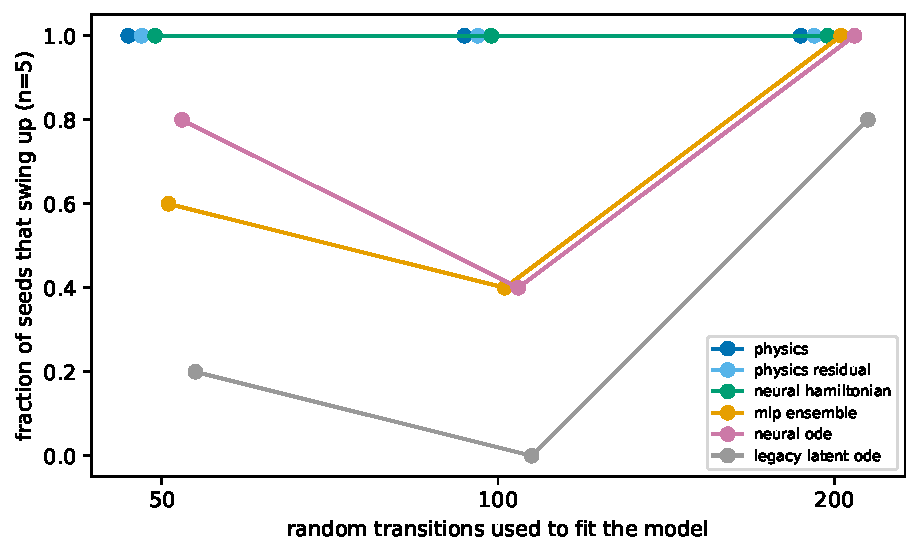
\includegraphics[width=0.62\textwidth]{fig2_lowdata.pdf}
\caption{Fraction of seeds (out of five) that swing the pendulum up when the model is fitted on only 50, 100 or 200 random transitions.}
\label{fig:low}
\end{figure}

\begin{table}[H]
\centering\small
\begin{tabular}{lccc}
\toprule
\tabL
\bottomrule
\end{tabular}
\caption{Seeds solved out of five, with the mean return $\bar R$, after fitting on very few random transitions (source: \texttt{results/phase\_d\_lowdata\_pendulum.json}).}
\label{tab:L}
\end{table}

\subsection{Changed physics and adaptation (H2)}
Figure~\ref{fig:shift} shows return in shifted worlds, on the left with the models unchanged and on the right after adapting with fifty transitions. Without adaptation every model loses a lot when gravity grows (around $-1260$ at gravity times $1.5$ against an oracle near $-434$). With fifty transitions every model recovers most of the gap.

\begin{figure}[H]
\centering
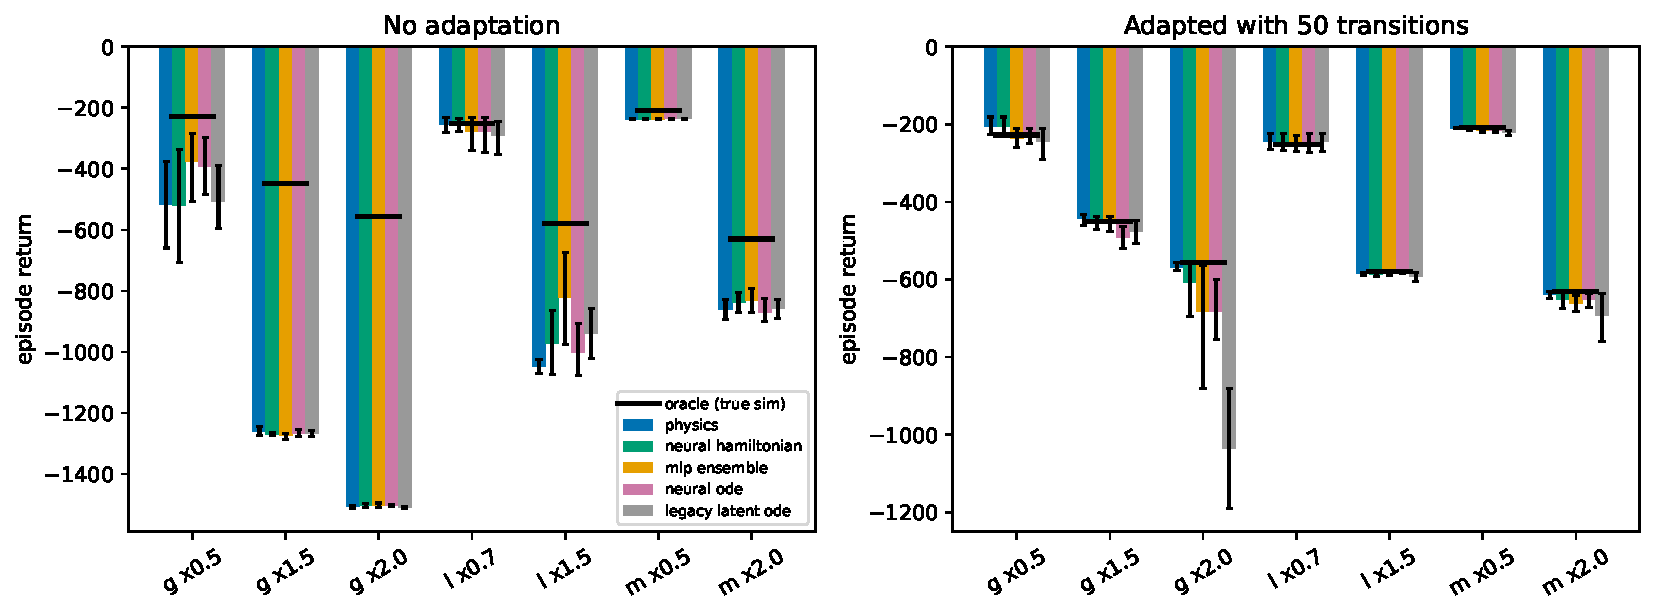
\includegraphics[width=\textwidth]{fig4_shift_returns.pdf}
\caption{Mean return per shift with 95\% bootstrap intervals over five seeds. Black ticks mark the oracle that plans with the true shifted simulator. Left: no adaptation. Right: after adaptation with 50 new transitions.}
\label{fig:shift}
\end{figure}

\begin{table}[H]
\centering\scriptsize
\resizebox{\textwidth}{!}{%
\begin{tabular}{lcccccccc}
\toprule
\tabEa
\bottomrule
\end{tabular}}
\caption{Mean return after adaptation with 50 transitions for each shift, with the oracle and the unadapted physics model for reference (source: \texttt{results/phase\_e\_pendulum.json}). For gravity times 2, length times 1.5 and mass times 2 even the oracle scores below $-500$, because swing up is slow under the torque limit.}
\label{tab:E}
\end{table}

The honest reading is this. After adaptation the physics model is nominally best at gravity times $1.5$ ($-443$, interval $[-461,-431]$ against $-456$, interval $[-474,-438]$, for the MLP ensemble), but the intervals of the physics model, the neural Hamiltonian and the MLP ensemble overlap, and for most shifts all models are within a few percent of the oracle. Return is a blunt instrument here because MPPI replans at every step and corrects errors of the size a fine tuned black box makes.

The prediction error tells a much sharper story (Figure~\ref{fig:needed}, Table~\ref{tab:E2}). After adaptation with fifty transitions the physics model predicts twenty five steps ahead with an error near $10^{-10}$ in every shift. The black boxes are between $10^{-3}$ and $10^{-1}$ at fifty transitions, and even with one thousand transitions none of them reached the physics model's fifty transition error. This is the strongest evidence for H2, and also where the caveat about the best case applies most: the structure is exactly correct and the data are noise free, so the physics model can only fail by having wrong constants.

\begin{figure}[H]
\centering
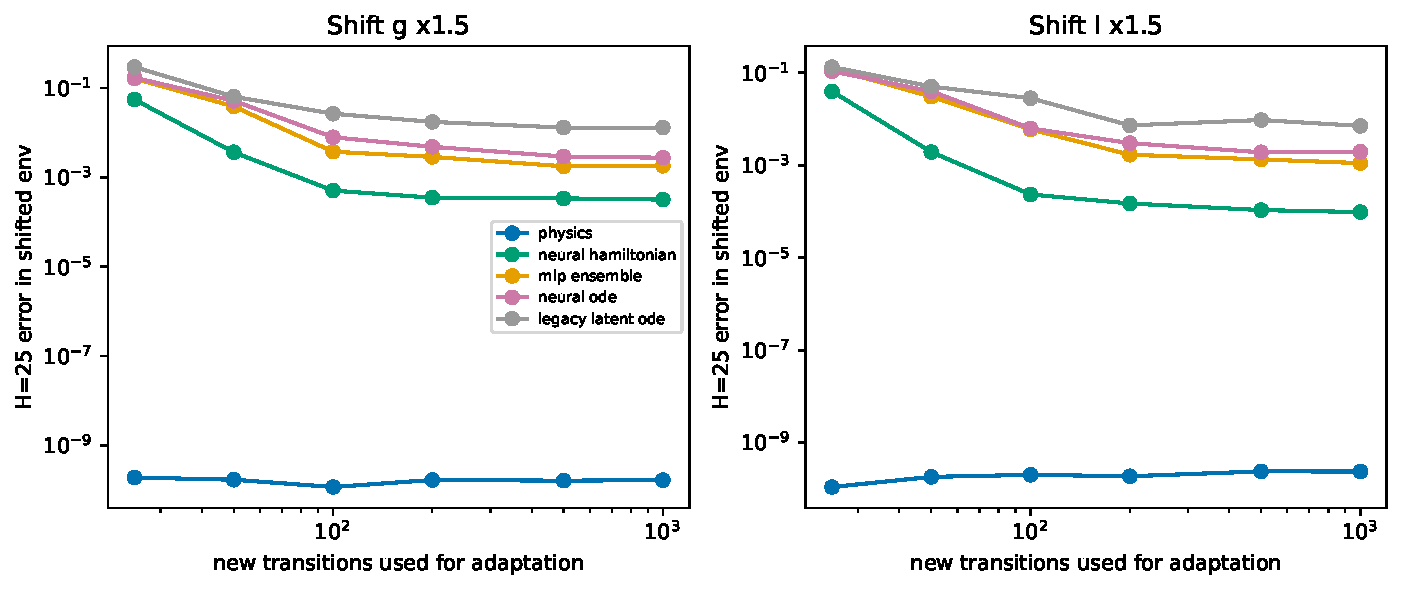
\includegraphics[width=\textwidth]{fig5_transitions_needed.pdf}
\caption{Median error twenty five steps ahead in the shifted world against the number of new transitions used for adaptation, for gravity times $1.5$ (left) and length times $1.5$ (right), five seeds.}
\label{fig:needed}
\end{figure}

\begin{table}[H]
\centering\small
\begin{tabular}{lcccccc}
\toprule
\tabEb
\bottomrule
\end{tabular}
\caption{Median prediction error at horizon 25 in the world with gravity times 1.5, against the number of adaptation transitions (columns).}
\label{tab:E2}
\end{table}

Figure~\ref{fig:recovery} shows parameter recovery. Over \recovN{} adaptation runs the median relative error of $a=3g/(2l)$ was \recovAmed{} (largest \recovAmax{}) and of $c=3/(ml^2)$ was \recovCmed{} (largest \recovCmax{}). I do not report separate estimates of $g$, $m$ and $l$ because they are not identifiable (Section~2.2). In an early version of my analysis I tabulated estimates of $g$ against the true shifted gravity, saw they disagreed, and realised that the learned mass and length sit on the non identifiable family, so that comparison was meaningless. I removed it and logged the mistake. Adapting only the one parameter that really changed gave the same return as adapting all of them ($-443.4$ against $-443.3$ at gravity times $1.5$).

\begin{figure}[H]
\centering
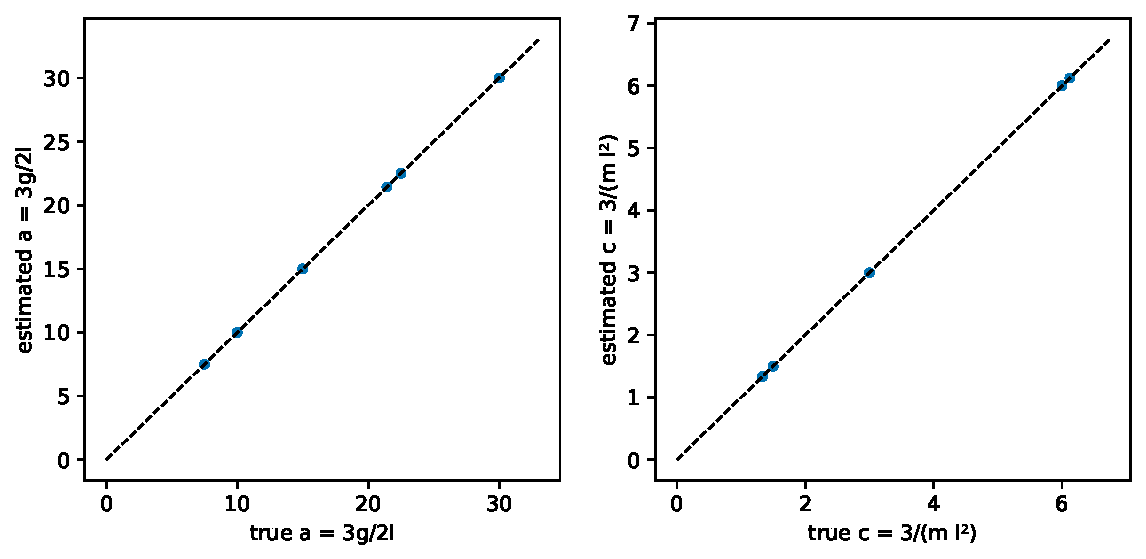
\includegraphics[width=0.85\textwidth]{fig6_param_recovery.pdf}
\caption{Estimated against true values of the identifiable combinations $a=3g/(2l)$ and $c=3/(ml^2)$ after adaptation with 50 transitions. The dashed line is perfect recovery.}
\label{fig:recovery}
\end{figure}

\subsection{Where the physics prior fails (H4)}
In the world with friction and a hidden motor limit (Figure~\ref{fig:fric}, Table~\ref{tab:F}) the physics model without a friction term has a twenty five step error of $0.28$, and so does the neural Hamiltonian ($0.27$), which has no dissipation term either. A learned residual brings the physics model to $0.0062$, about forty five times better. But the MLP ensemble reaches $0.0071$ without any physics at all, so the residual repairs the structured model to the level of a plain network and does not beat it. Giving the physics model a learnable friction coefficient helps only partly (error $0.08$, with $b$ estimated between $0.06$ and $0.16$ against a true value of $0.15$) because the hidden motor limit is still unmodelled.

\begin{figure}[H]
\centering
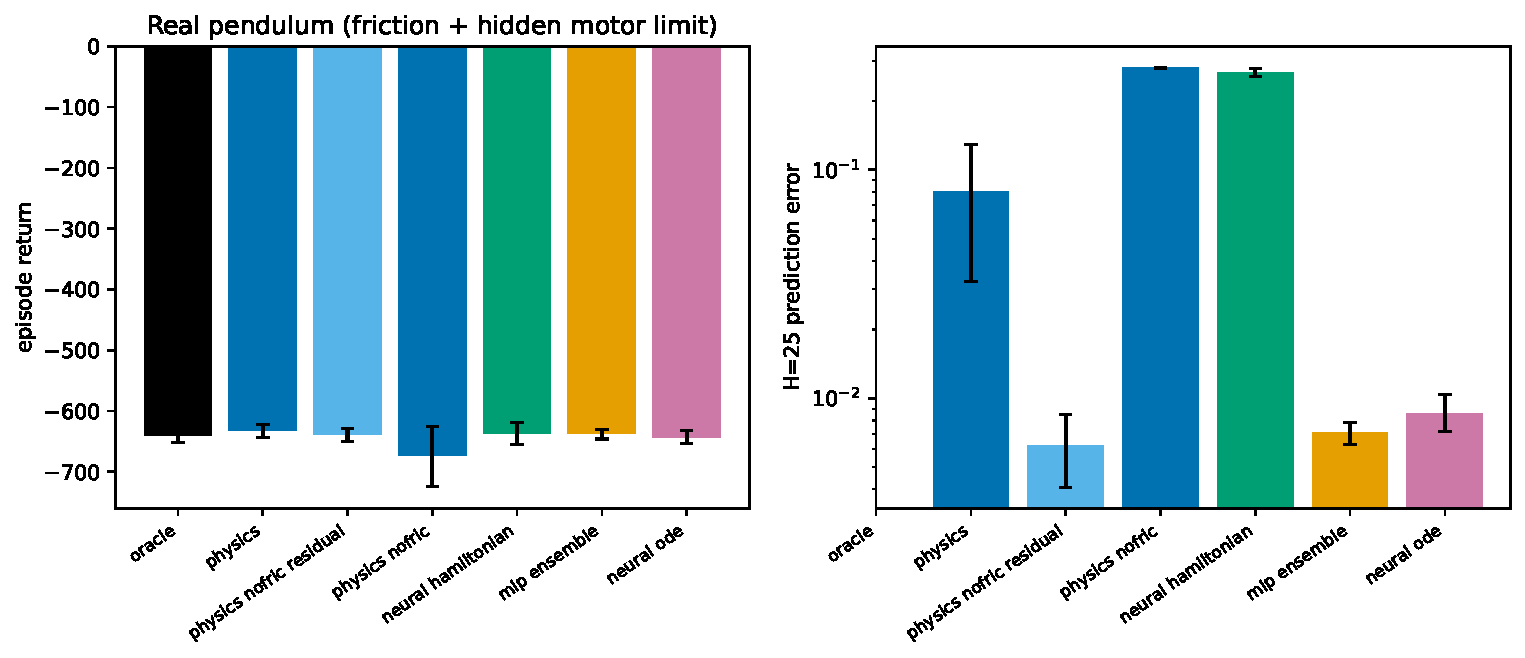
\includegraphics[width=\textwidth]{fig7_friction_failure.pdf}
\caption{The real pendulum with viscous friction and a hidden motor limit. Left: return in the last three episodes. Right: error twenty five steps ahead (log scale). Bars show means over five seeds with 95\% bootstrap intervals.}
\label{fig:fric}
\end{figure}

\begin{table}[H]
\centering\small
\begin{tabular}{lcc}
\toprule
\tabF
\bottomrule
\end{tabular}
\caption{Results in the world with friction and a hidden motor limit (source: \texttt{results/phase\_f\_pendulum.json}).}
\label{tab:F}
\end{table}

In return, every agent ends within noise of the oracle ($-640$). Only the physics model without friction is nominally lower ($-673$) and its interval overlaps the others. So H4 is supported for prediction and invisible in return, for the same reason as before.

\subsection{Demonstration}
The script \texttt{demo/make\_gif.py} produces \texttt{figures/demo\_shifted\_gravity.gif}, a ten second side by side episode at gravity times $1.5$ with seed zero. The unadapted MLP scores $-1280$, the adapted MLP scores $-498$ and the adapted physics model scores $-497$. The animation is a fair picture of the whole study: adaptation matters a great deal, and in this episode the adapted black box swings up just as well. The difference between the models is in the quality of the predictions, not in this outcome.

\subsection{Verdict on the hypotheses}
\begin{table}[H]
\centering\small
\begin{tabular}{p{1.2cm}p{3.1cm}p{9.4cm}}
\toprule
 & Verdict & Evidence \\
\midrule
H1 & Weak, regime dependent & No difference at 500 or more random transitions. At 50 transitions the structured models solved 5 of 5 seeds against 1 to 4 of 5 for black boxes, but with five seeds and noisy counts. \\
H2 & Strong for prediction, weak for return & Prediction error after adaptation near $10^{-10}$ against $10^{-3}$ to $10^{-1}$ for black boxes. Returns after adaptation are all close to the oracle with overlapping intervals. \\
H3 & Supported & Physics, then neural Hamiltonian, then MLP ensemble, then neural ODE, then legacy at every horizon. Hamiltonian energy drift stays flat. \\
H4 & Supported for prediction, not visible in return & Error $0.28$ without a friction term, $0.006$ with a residual (about the same as an MLP). Returns within noise of the oracle. \\
\bottomrule
\end{tabular}
\caption{Summary of the four hypotheses.}
\end{table}

%--------------------------------------------------------------------
\section{What went wrong along the way}
I kept a bug log while working, and these are the lessons that mattered.
\begin{enumerate}[leftmargin=1.8em]
\item \textbf{Energy drift that looked like a physics bug.} The first energy test failed. A sweep over the number of substeps showed the error falling by thirty two times per halving, which pointed at RK4 truncation and not at the equations. Lesson: check the convergence order before blaming the physics.
\item \textbf{Precision loss from mixed dtypes.} A test built the action in single precision against a double precision state and lost about $10^{-8}$. Lesson: keep one dtype everywhere.
\item \textbf{A reference that did not use the same discretisation.} After adding substeps, the NumPy comparison used one step and the simulator used four. The test was wrong, not the simulator.
\item \textbf{A commit with failing tests.} A shell edit failed silently and I committed Phase A with three failing tests, then fixed it in the next commit. Lesson: run the tests before committing.
\item \textbf{A leak I caught in review.} The physics model would have started its friction coefficient at the true value in the friction experiment. I changed it to start at zero before running that experiment.
\item \textbf{Tests that could not fail.} An interquartile mean test passed vacuously twice, first because its outliers cancelled in the mean and then because my text replacement did not match. Lesson: make sure a test would fail on a broken implementation.
\item \textbf{A misleading table row} comparing estimated gravity against the true shifted value, explained above.
\item \textbf{The main sweep did not discriminate.} All models solved the task at five hundred transitions. I added the low data sweep afterwards and said so.
\end{enumerate}

%--------------------------------------------------------------------
\section{Limitations and threats to validity}
\begin{itemize}[leftmargin=1.5em]
\item The simulator is noise free, the state is fully observed, and the structured model contains the true equations. This is the best case for physics models. A real robot has noise, partial observation, contacts and unmodelled effects.
\item Learning experiments use the pendulum only. I make no claim about the cart pole or the acrobot beyond the tests of the simulators and the planner.
\item Five seeds and many comparisons without a multiple comparison correction. Bootstrap intervals over five points are rough.
\item One hyperparameter setting per model. The black boxes might improve with a multi step loss, a likelihood loss, or more tuning, and the legacy model has less capacity.
\item Return saturates because of replanning, so conclusions based on return are weaker than conclusions based on prediction.
\item Shared start states and planner seeds make returns highly correlated across models, which makes ties look exact.
\item SAC was run for ten thousand steps and two of five seeds had not converged, so the statement that model based control is about ten times more sample efficient is a rough, single environment statement.
\item I did not record the total wall clock time of the full sweep. The Phase D jobs alone add up to about 83{,}000 CPU seconds (about 3.3 hours on seven workers, of which 53\% was the neural Hamiltonian), and the other phases came on top. The full sweep may therefore exceed the six hour budget I set myself. The reduced fast reproduction mode has not been timed or validated end to end.
\end{itemize}

%--------------------------------------------------------------------
\section{Relation to earlier work and what is new}
\label{sec:related}
The neural Hamiltonian with control follows Symplectic ODE Net~\cite{zhong2020symoden}, which builds on Hamiltonian neural networks~\cite{greydanus2019hnn}. Lagrangian neural networks~\cite{cranmer2020lnn} and Deep Lagrangian Networks~\cite{lutter2019delan} are related approaches that I did not implement. The ensemble model is a simplified version of PETS~\cite{chua2018pets}. The residual is inspired by APHYNITY~\cite{yin2021aphynity} without its constrained optimisation. The planner is MPPI~\cite{williams2017mppi,williams2016aggressive}, and TD MPC~\cite{hansen2022tdmpc} is a learned latent alternative that I did not try. The method ideas here are not new. What I can claim is a careful and reproducible small comparison, a clean demonstration of the identifiability problem, and the observation that replanning hides model error when performance is measured by return. I would not present this as new research.

%--------------------------------------------------------------------
\section{Next steps}
\begin{itemize}[leftmargin=1.5em]
\item Run the same pipeline on the cart pole and the acrobot, then add observation noise and partial observation.
\item Train black boxes with a multi step loss and a likelihood loss, and fix the Hamiltonian model's mass matrix to see how much of its accuracy comes from learning it.
\item Use more seeds (ten or more) and a matched compute comparison with SAC.
\item Choose the adaptation transitions instead of drawing them at random. With ensemble disagreement, or the width of the parameter estimate for the structured model, one could pick the fifty transitions that excite $a$ and $c$ the most. This connects to a question I find interesting: how much does which experience an agent collects matter, for the same world models?
\end{itemize}

%--------------------------------------------------------------------
\appendix
\section{Reproduction}
From the repository root, with Python 3.13, PyTorch 2.12, NumPy 2.3, Gymnasium 1.4, torchdiffeq 0.2.5, pytorch\_mppi 0.9.1 and rliable 1.2.0 (see \texttt{requirements.txt}):
\begin{itemize}[leftmargin=1.5em]
\item \texttt{make test} runs the 38 control tests and the original orbit test in about half a minute.
\item \texttt{make phase\_c}, \texttt{make phase\_d}, \texttt{make phase\_d\_lowdata}, \texttt{make phase\_e} and \texttt{make phase\_f} regenerate the raw results in \texttt{results/}. Phase E needs the models that Phase D saves in \texttt{results/models/}, which is not tracked by git.
\item \texttt{make report\_figs} regenerates all figures and \texttt{results/summary\_table.md}.
\item \texttt{make report} regenerates the tables of this report and compiles \texttt{docs/report\_control/report\_control.tex} into this PDF (it needs the \texttt{tectonic} LaTeX engine).
\item \texttt{make demo} makes the demonstration animation.
\item \texttt{make repro\_fast} chains a reduced version of everything (two seeds, shorter runs); it has not been timed.
\end{itemize}

\section{Study questions}
These are the questions I used to check my own understanding. Short answers follow.
\begin{enumerate}[leftmargin=1.8em]
\item Why does a Hamiltonian model conserve energy when the control is zero, even if its learned $H$ is wrong?
\item Why are only $a=3g/(2l)$ and $c=3/(ml^2)$ identifiable for the pendulum?
\item What does the temperature $\lambda$ do in MPPI, and what happens as it goes to zero or to infinity?
\item Why does model predictive control hide some model error?
\item Why must the validation split be made by episode?
\item Why does a learned residual hurt on clean data but help in the friction world?
\item Why can the neural Hamiltonian here not model friction?
\item Why are returns nearly identical across models in the main sweep?
\item The physics model reaches an error of $10^{-10}$. Is that suspicious, and what makes it plausible?
\item What would you change to test whether the Hamiltonian result comes from the learned mass matrix?
\end{enumerate}
\textbf{Answers.}
(1) Because $dH/dt=\partial_q H\,\dot q+\partial_p H\,\dot p=0$ for any $H$ when $\dot q=\partial_p H$ and $\dot p=-\partial_q H$. The learned energy is conserved, though it may differ from the true energy.
(2) The dynamics depend on $g$ and $l$ only through $g/l$, and on $m$ and $l$ only through $ml^2$, so there are three unknowns and two constraints.
(3) It sets how sharply the plan follows the best samples. As $\lambda\to0$ it copies the best sample, and as $\lambda\to\infty$ it averages all samples.
(4) Each replan starts from the observed true state, so small errors do not accumulate over the whole episode.
(5) Rows from one episode are strongly correlated, so a row level split leaks information into validation.
(6) With nothing missing the residual only adds capacity and noise. With friction and saturation missing it has something real to capture.
(7) Its momentum equation has no dissipative term, so its flow cannot lose energy.
(8) The agents share start states and planner seeds, and all models are accurate enough for the same actions to be chosen.
(9) It is plausible only because the simulator is noise free and the structure is exactly right, so only the constants are unknown. It would not hold on real data.
(10) Fix the inverse mass matrix to the true $3/(ml^2)$ and compare accuracy.

\section{Exercises}
\begin{enumerate}[leftmargin=1.8em]
\item Run the demonstration at gravity times $0.5$ and predict first which agents will swing up fastest.
\item Cut the MPPI horizon from forty to fifteen steps and predict what happens on the pendulum (the torque limit forces several swings).
\item Swap the CEM planner into the control loop and compare time and return.
\item Add observation noise to the collected data and see how the gap between physics and black boxes changes.
\item Train the black boxes with a five step unrolled loss and see whether the horizon gap narrows.
\item Fix the Hamiltonian model's mass matrix to the true one and measure the change.
\item Run the shifted physics pipeline on the cart pole, where the parameters may be fully identifiable.
\item Add the acrobot to the structured model and check energy drift on a chaotic system.
\end{enumerate}

%--------------------------------------------------------------------
\begin{thebibliography}{99}\small
\bibitem{zhong2020symoden} Y. D. Zhong, B. Dey, A. Chakraborty. Symplectic ODE Net: Learning Hamiltonian dynamics with control. \emph{International Conference on Learning Representations (ICLR)}, 2020. arXiv:1909.12077.
\bibitem{chen2018neuralode} R. T. Q. Chen, Y. Rubanova, J. Bettencourt, D. Duvenaud. Neural ordinary differential equations. \emph{Advances in Neural Information Processing Systems (NeurIPS)}, 2018. arXiv:1806.07366.
\bibitem{greydanus2019hnn} S. Greydanus, M. Dzamba, J. Yosinski. Hamiltonian neural networks. \emph{NeurIPS}, 2019. arXiv:1906.01563.
\bibitem{cranmer2020lnn} M. Cranmer, S. Greydanus, S. Hoyer, P. Battaglia, D. Spergel, S. Ho. Lagrangian neural networks. \emph{ICLR Workshop on Integration of Deep Neural Models and Differential Equations}, 2020. arXiv:2003.04630.
\bibitem{lutter2019delan} M. Lutter, C. Ritter, J. Peters. Deep Lagrangian networks: Using physics as model prior for deep learning. \emph{ICLR}, 2019. arXiv:1907.04490.
\bibitem{chua2018pets} K. Chua, R. Calandra, R. McAllister, S. Levine. Deep reinforcement learning in a handful of trials using probabilistic dynamics models. \emph{NeurIPS}, 2018. arXiv:1805.12114.
\bibitem{yin2021aphynity} Y. Yin, V. Le Guen, J. Dona, E. de Bezenac, I. Ayed, N. Thome, P. Gallinari. Augmenting physical models with deep networks for complex dynamics forecasting. \emph{ICLR}, 2021. arXiv:2010.04456.
\bibitem{williams2017mppi} G. Williams, N. Wagener, B. Goldfain, P. Drews, J. M. Rehg, B. Boots, E. A. Theodorou. Information theoretic MPC for model based reinforcement learning. \emph{IEEE International Conference on Robotics and Automation (ICRA)}, 2017.
\bibitem{williams2016aggressive} G. Williams, P. Drews, B. Goldfain, J. M. Rehg, E. A. Theodorou. Aggressive driving with model predictive path integral control. \emph{ICRA}, 2016.
\bibitem{hansen2022tdmpc} N. Hansen, X. Wang, H. Su. Temporal difference learning for model predictive control. \emph{International Conference on Machine Learning (ICML)}, 2022. arXiv:2203.04955.
\bibitem{haarnoja2018sac} T. Haarnoja, A. Zhou, P. Abbeel, S. Levine. Soft actor critic: Off policy maximum entropy deep reinforcement learning with a stochastic actor. \emph{ICML}, 2018. arXiv:1801.01290.
\bibitem{huang2022cleanrl} S. Huang, R. F. J. Dossa, C. Ye, J. Braga, D. Chakraborty, K. Mehta, J. G. M. Araujo. CleanRL: High quality single file implementations of deep reinforcement learning algorithms. \emph{Journal of Machine Learning Research}, 23(274), 2022.
\bibitem{towers2024gymnasium} M. Towers et al. Gymnasium: A standard interface for reinforcement learning environments. arXiv:2407.17032, 2024.
\bibitem{agarwal2021precipice} R. Agarwal, M. Schwarzer, P. S. Castro, A. Courville, M. G. Bellemare. Deep reinforcement learning at the edge of the statistical precipice. \emph{NeurIPS}, 2021. arXiv:2108.13264.
\bibitem{efron1979bootstrap} B. Efron. Bootstrap methods: Another look at the jackknife. \emph{The Annals of Statistics}, 7(1):1 to 26, 1979.
\bibitem{kingma2015adam} D. P. Kingma, J. Ba. Adam: A method for stochastic optimization. \emph{ICLR}, 2015. arXiv:1412.6980.
\bibitem{goldstein2002} H. Goldstein, C. Poole, J. Safko. \emph{Classical Mechanics}, third edition. Addison Wesley, 2002.
\bibitem{pytorchmppi} University of Michigan ARM Lab. pytorch\_mppi: Model predictive path integral control in PyTorch. Software, \url{https://github.com/UM-ARM-Lab/pytorch_mppi}.
\end{thebibliography}

\end{document}
